\section{Wstęp}
W dzisiejszym globalnym świecie znajomość języków obcych jest nieocenioną umiejętnością. Tradycyjne metody nauki, takie jak lekcje w klasach, samouczki i aplikacje do nauki słownictwa, często są czasochłonne i nie zawsze dostosowane do indywidualnych potrzeb ucznia. Dodatkowo, oglądanie filmów i seriali w obcym języku jest powszechnie uznawane za skuteczny sposób na poprawę umiejętności językowych, ale brakuje narzędzi, które integrują te aktywności z formalnym procesem nauki. Niniejsza praca inżynierska koncentruje się na stworzeniu innowacyjnej aplikacji webowej, która połączy te dwa aspekty, oferując użytkownikom skuteczniejsze i przyjemniejsze doświadczenie edukacyjne.

Współczesny świat, w którym żyjemy, jest coraz bardziej zglobalizowany i wymaga od nas umiejętności komunikacji w różnych językach, a przede wszystkim w języku angielskim, który stał się międzynarodowym językiem na świecie. Wraz z rozwojem technologii, nauka języków obcych stała się bardziej dostępna i atrakcyjna. Znajomość języków obcych nie tylko otwiera drzwi do nowych możliwości zawodowych, ale także umożliwia pełniejsze zrozumienie innych kultur i poszerza horyzonty. Wraz z dynamicznym rozwojem technologii, nauka języków obcych stała się bardziej dostępna, a tradycyjne metody nauczania ewoluowały, oferując nowe, bardziej interaktywne formy edukacji. Jednym z najpopularniejszych sposobów nauki języków jest korzystanie z platform internetowych, takich jak duoLingo, gdzie użytkownicy mogą uczyć się od podstaw słów i zdań które zostały wcześniej przygotowane. Jednakże, nauka języka obcego w ten sposób ogranicza nas w kwesti wyboru czego chcielisbyśmy się dokładnie uczyć.

Coraz więcej osób szuka alternatywnych metod nauki, które są bardziej angażujące i interaktywne. Filmy i seriale oferują naturalny kontekst, w którym używane są różne zwroty i słownictwo, co czyni je doskonałym narzędziem do nauki języka. Oglądanie treści w języku obcym nie tylko pomaga w nauce nowych słów i zwrotów, ale także w poprawie umiejętności słuchania i rozumienia języka w różnych akcentach i dialektach.

Aplikacja ta ma umożliwić użytkownikom aktywne uczestnictwo w procesie nauki, poprzez interaktywne narzędzia i funkcje, które wspomagają naukę słownictwa i gramatyki. Wśród nich znajdują się m.in. możliwość zapisu słów z listy napisów, które są wyświetlane pod lub obok odtwarzacza video, a także możliwość dodania ich do bazy danych, aby uniknąć powtórzeń baza nie przyjmie drugiego takiego samego słowa użytkownikowi. Użytkownik będzie miał dostęp do panelu nauki, słownika wszystkich słów, możliwości logowania z różnych urządzeń obsługujących przeglądarkę, a także do różnych sposobów nauki, takich jak słownik, flashcards, quiz czy lista napisów.

Aplikacja ta ma również uwzględnić elementy gamifikacji, aby zachęcić użytkowników do nauki i śledzenia postępów. Na profilu użytkownika będą widoczne wszystkie nauczone słowa, a także osobna podstrona z wykresami i informacjami o postępach. Dzięki tej aplikacji, użytkownicy będą mogli efektywnie i atrakcyjnie uczyć się języka obcego, korzystając z platformy YouTube i własnych filmów z napisami z dysku własnego komputera. Napisy których użytkownik może użyć będą w różnych formatach, więc w aplikacji będzię można wybrać rodzaj pliku i przekopiować całą zawartość lub wrzucić plik w odpowiednie miejsce, napisy muszą zostać zapisane w systemie ponieważ nie ma możliwośći zapisaniu scieżki do żadnego pliku ze względów bezpieczeństwa w internecie.

Wybór technologii do tworzenia aplikacji webowej jest kluczowy dla jej stabilności, skalowalności i wydajności. W projekcie tej aplikacji językowej zdecydowano się na framework Next.js, który oparty jest na React i oferuje wiele korzyści. Jedną z głównych zalet Next.js jest możliwość elastycznego renderowania treści, zarówno po stronie serwera (SSR), jak i klienta (CSR). Dzięki SSR, aplikacja może szybko ładować wstępnie załadowane strony, co znacząco poprawia widoczność w wyszukiwarkach (SEO - Search Engine Optimization) i przyspiesza czas ładowania, co jest szczególnie istotne dla użytkowników korzystających z platformy edukacyjnej. CSR z kolei umożliwia dynamiczne i płynne aktualizacje interfejsu bez konieczności przeładowywania całej strony, co poprawia doświadczenie użytkownika.


\section{Przegląd aktualnych rozwiązań}

\subsection{Anki}
Anki to popularna aplikacja edukacyjna oparta na systemie powtórek rozłożonych w czasie (Spaced Repetition System – SRS). Dzięki temu mechanizmowi nauka jest bardziej efektywna, ponieważ aplikacja prezentuje użytkownikowi informacje w odpowiednich odstępach czasowych, co pomaga w utrwaleniu materiału. Anki wyróżnia się uniwersalnością i możliwością dostosowania do różnych potrzeb, takich jak nauka języków obcych, przygotowanie do egzaminów czy zapamiętywanie faktów w innych dziedzinach.\\
\textbf{Funkcjonalności}:
\begin{itemize}
    \item Możliwość ręcznego dodawania kart z różnymi typami treści, w tym tekstów, obrazów, dźwięków i nagrań wideo.
    \item Obsługa dodatków (pluginów), które rozszerzają możliwości aplikacji, np. importowanie napisów filmowych.
    \item Analiza postępów użytkownika z wykorzystaniem statystyk i wykresów.
\end{itemize}
\textbf{Ograniczenia}:
\begin{itemize}
    \item Podczas oglądania filmu użytkownik musi ręcznie przerywać oglądanie, aby dodawać niezbędne informacje do kart. Utrudnia to płynność procesu i może obniżać komfort nauki.
    \item Mimo tych niedogodności Anki pozostaje dobrym rozwiązaniem do nauki języków, szczególnie dzięki możliwości personalizacji kart i śledzenia postępów.
\end{itemize}
\begin{figure}[H]
    \centering
    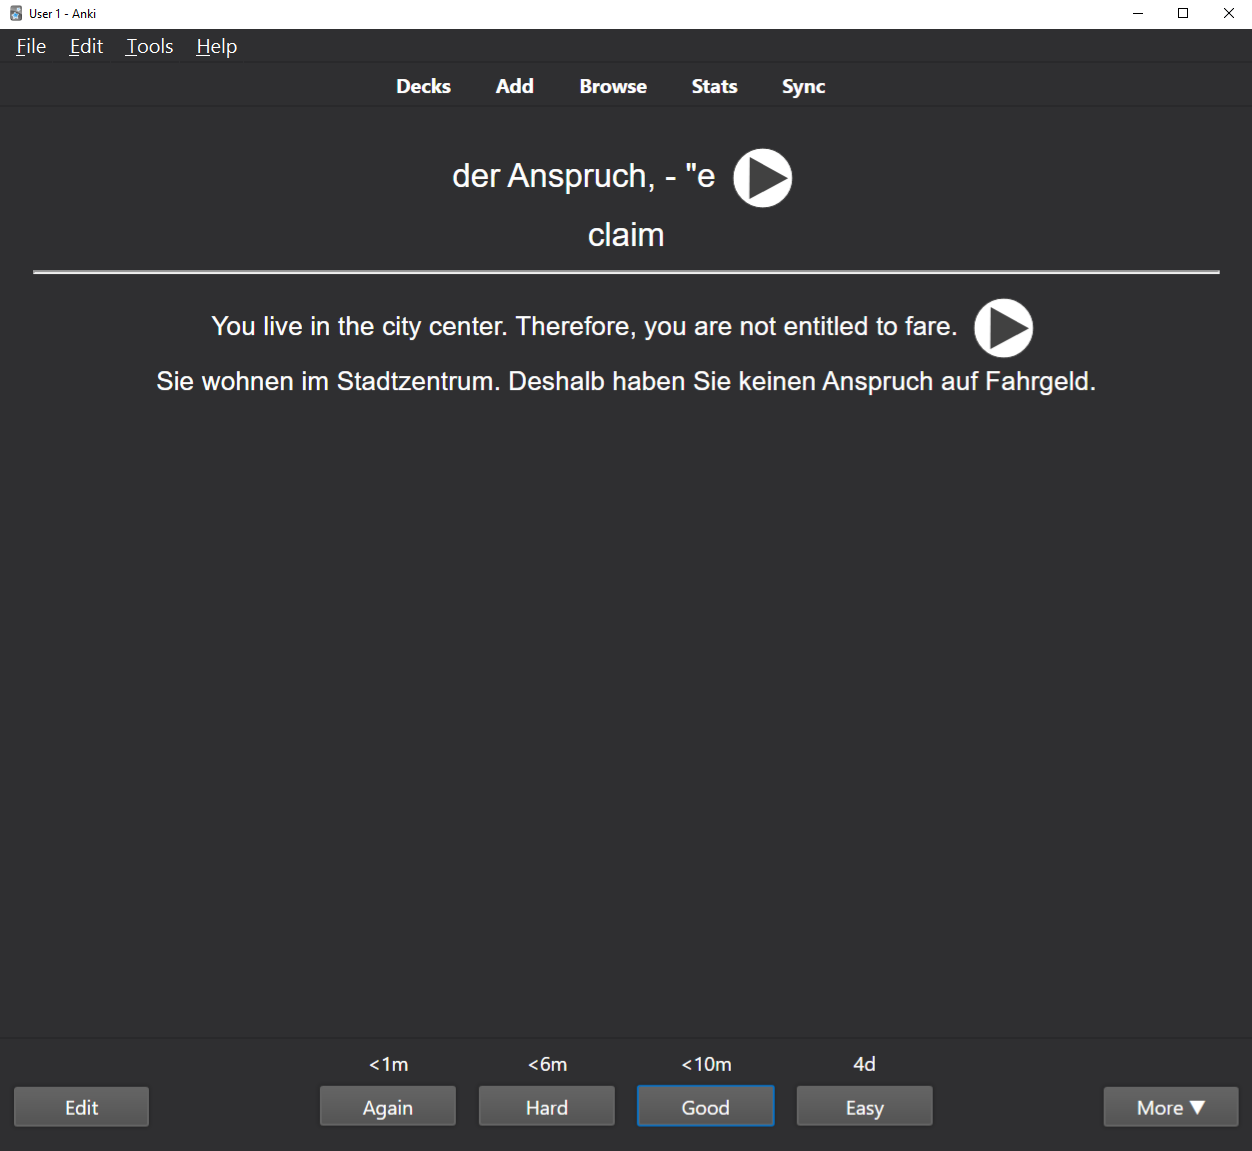
\includegraphics[width=0.8\textwidth]{IMAGE/Anki.png}
    \caption{Nauka słówek w aplikacji Anki}
    \label{fig:Anki}
\end{figure}
\subsection{Language Reactor}
Language Reactor to narzędzie edukacyjne, które umożliwia naukę języków obcych w sposób przyjemny i efektywny poprzez oglądanie filmów i seriali. Aplikacja oferuje interaktywne napisy, które umożliwiają tłumaczenie słów i zwrotów bezpośrednio na ekranie. Dzięki tej funkcji użytkownicy mogą szybko sprawdzić znaczenie nowego słowa, klikając na nie podczas oglądania, lub oznaczyć jako słowo do nauki, ale jest to możliwe dopiero po zapłaceniu za usługę “pro” na stronie. \\
\textbf{Funkcjonalności}:
\begin{itemize}
    \item {\textbf{Interaktywne napisy}}: Jedną z głównych zalet Language Reactor jest możliwość wyświetlania tłumaczeń słów i zwrotów w trakcie oglądania, co sprawia, że nauka odbywa się w naturalnym kontekście. Dzięki temu użytkownik może natychmiast zobaczyć, jak dane słowo funkcjonuje w zdaniu.
    \item {\textbf{Integracja z platformami streamingowymi}}: Aplikacja działa z popularnymi serwisami, takimi jak YouTube, Netflix czy Disney+, co oznacza, że użytkownicy mogą korzystać z niej podczas oglądania ulubionych filmów i seriali w obcym języku.
    \item {\textbf{Słownik i lematyzacja}}: Language Reactor automatycznie przetwarza słowa na ich formy podstawowe (lematy), co pomaga w nauce gramatyki oraz zapamiętywaniu nowych słówek bez względu na ich odmianę.
    \item {\textbf{Baza słówek}}: Użytkownicy mogą zapisywać słówka, które napotkali podczas oglądania, tworząc spersonalizowaną listę do późniejszego przyswajania. To rozwiązanie pozwala na systematyczną naukę i powtórki.
    \item {\textbf{System powtórek SRS}}: Aplikacja wprowadza system powtórek rozłożonych w czasie, co wspomaga długotrwałe zapamiętywanie materiału, podobnie jak w przypadku Anki.
    \item {\textbf{ifDostosowanie poziomu trudności}}: Użytkownicy mogą dostosować poziom trudności materiałów, co pozwala na naukę dostosowaną do ich umiejętności i tempa.
\end{itemize}

\textbf{Ograniczenia}:
\begin{itemize}
    \item \textbf{Ograniczona dostępność}: Language Reactor jest dostępny tylko na wybranych platformach streamingowych, co ogranicza możliwość korzystania z aplikacji do nauki języków z innych źródeł.
    \item \textbf{Płatne funkcje}: Pełna funkcjonalność aplikacji, w tym możliwość zapisywania słówek i korzystania z systemu powtórek, jest dostępna tylko w wersji płatnej, co może być barierą dla niektórych użytkowników.
\end{itemize}

\begin{figure}[H]
    \centering
    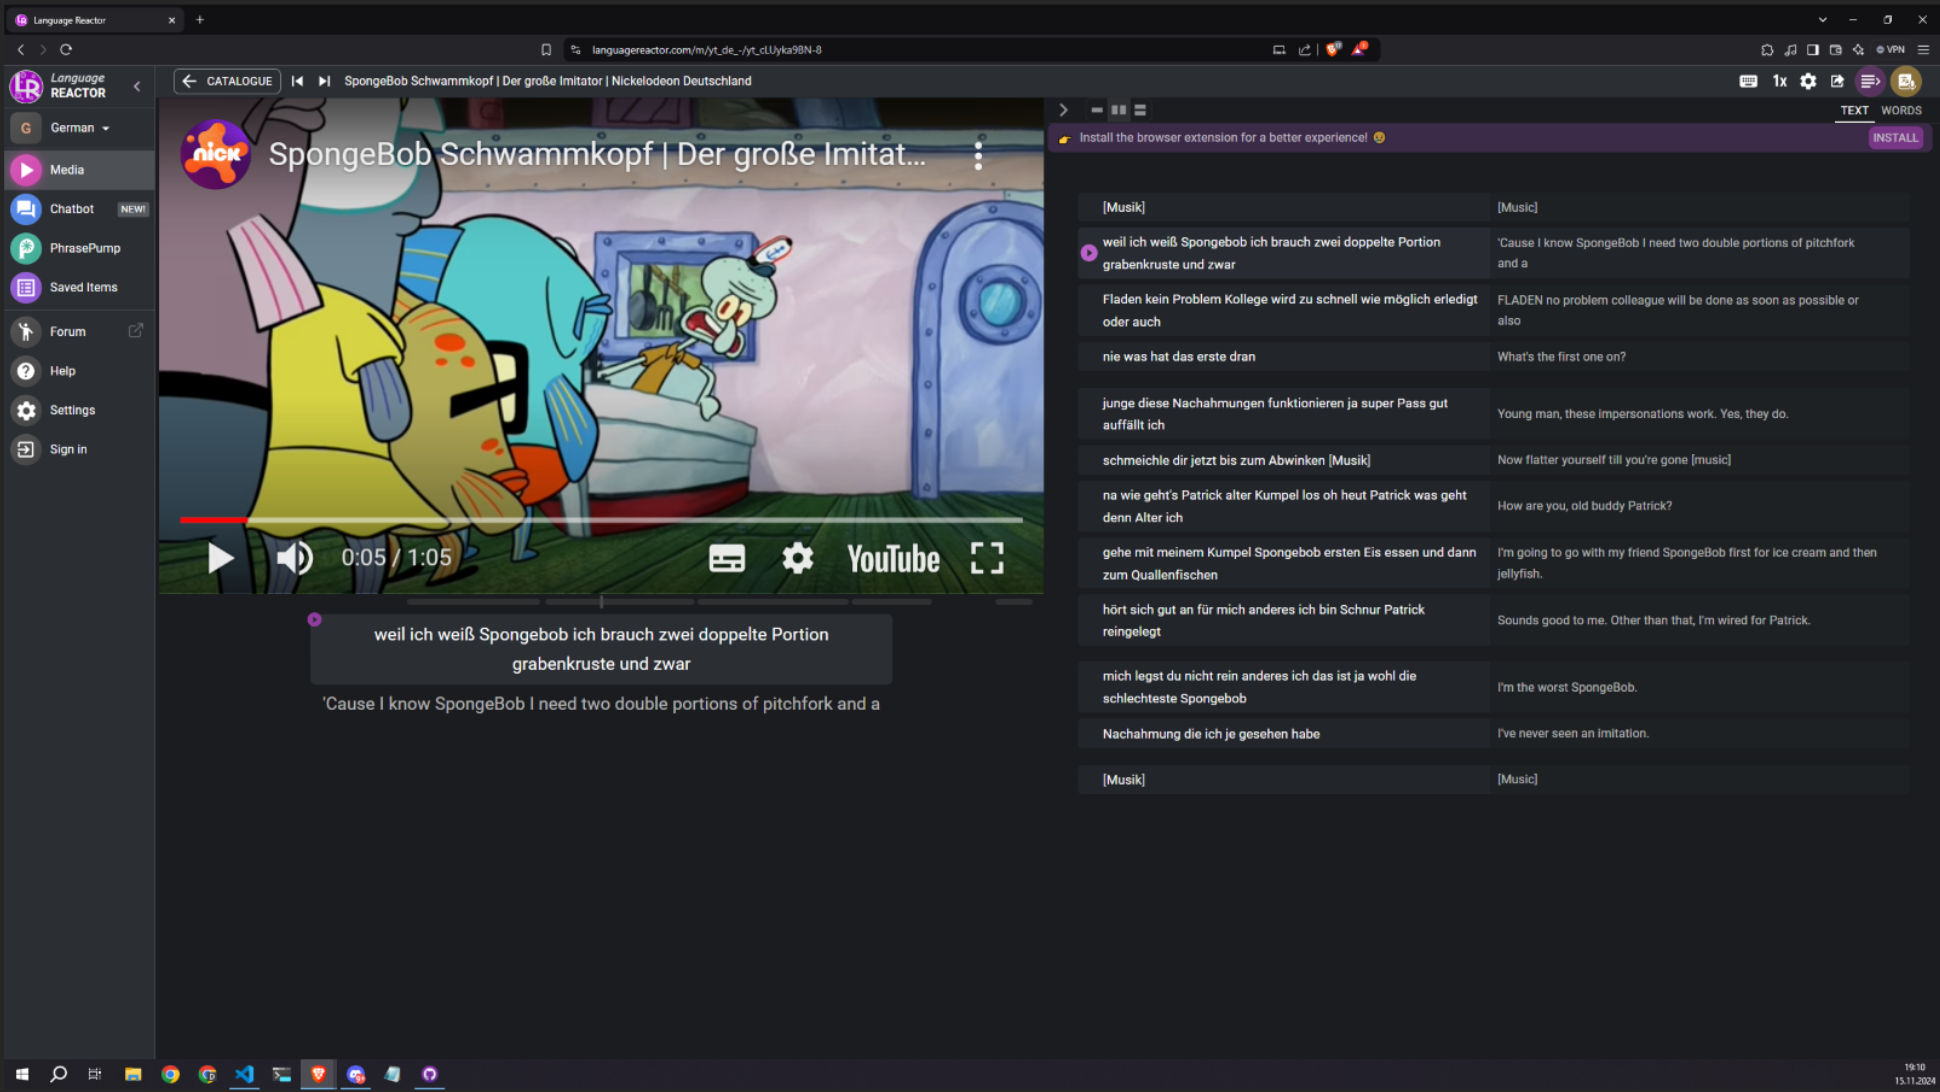
\includegraphics[width=0.8\textwidth]{IMAGE/LanguageReactor.png}
    \caption{Interaktywne napisy na stronie Language Reactor}
    \label{fig:Language_reactor}
\end{figure}

Możliwość nauki tylko z wybranych kanałów youtube nie można wybrać filmu który nie jest na liście strony internetowej.
\subsection{Trancy}
Trancy to aplikacja stworzona z myślą o nauce języków obcych, która integruje naukę słówek z oglądaniem filmów, seriali i innych materiałów wideo. Aplikacja oferuje funkcje, które pozwalają użytkownikom uczyć się języka poprzez interaktywne napisy, tłumaczenia oraz dodatkowe ćwiczenia, co sprawia, że proces nauki staje się bardziej angażujący i efektywny. \\
\textbf{Funkcjonalności}:
\begin{itemize}
    \item \textbf{Interaktywne napisy}: Trancy umożliwia wyświetlanie napisów w różnych językach, z tłumaczeniami słów i zwrotów. Dzięki temu użytkownicy mogą szybko zrozumieć, co oznacza dane słowo, a także zobaczyć je w kontekście. Napisy są dostosowane do poziomu zaawansowania użytkownika, co pozwala na naukę w sposób dostosowany do indywidualnych potrzeb.
    \item \textbf{Zbieranie słówek}: Użytkownicy mogą zapisywać napotkane słówka, które następnie mogą zostać przekształcone w fiszki do nauki. Taki system pozwala na systematyczne utrwalanie materiału i umożliwia szybkie powtórki w dogodnym czasie.
    \item \textbf{Tłumaczenia i definicje}: Aplikacja oferuje tłumaczenie słów na różne języki oraz wyświetlanie ich definicji, co wspomaga naukę gramatyki i budowanie słownictwa. Użytkownicy mogą korzystać z wbudowanego słownika, aby na bieżąco zgłębiać znaczenie nowych wyrazów.
    \item \textbf{Fiszki SRS}: Trancy wykorzystuje system powtórek rozłożonych w czasie (SRS), który pomaga w długotrwałym zapamiętywaniu słówek. Użytkownik dostaje powiadomienia o konieczności powtórki, co pozwala na regularne utrwalanie materiału i skuteczniejszą naukę.
\end{itemize}
\textbf{Ograniczenia}:
\begin{itemize}
    \item \textbf{Wymaga płatnej subskrypcji}: Aby w pełni skorzystać z funkcji aplikacji, użytkownik musi zapłacić, w wersji darmowej są tylko niezbędne narzędzia jak tłumaczenie i limit do 100 słów do zapisania.
    \item \textbf{Ograniczona integracja z platformami}: Trancy oferuje integrację z wybranymi platformami streamingowymi, i nie daje możliwości nauki z własnych zapisanych filmów.
    \item \textbf{Wymagana wtyczka w przeglądarce}: Żeby dodawać słowa lub oglądać filmy musimy robić to poza stroną Trancy z użyciem wtyczki Trancy.
\end{itemize}

\begin{figure}[H]
    \centering
    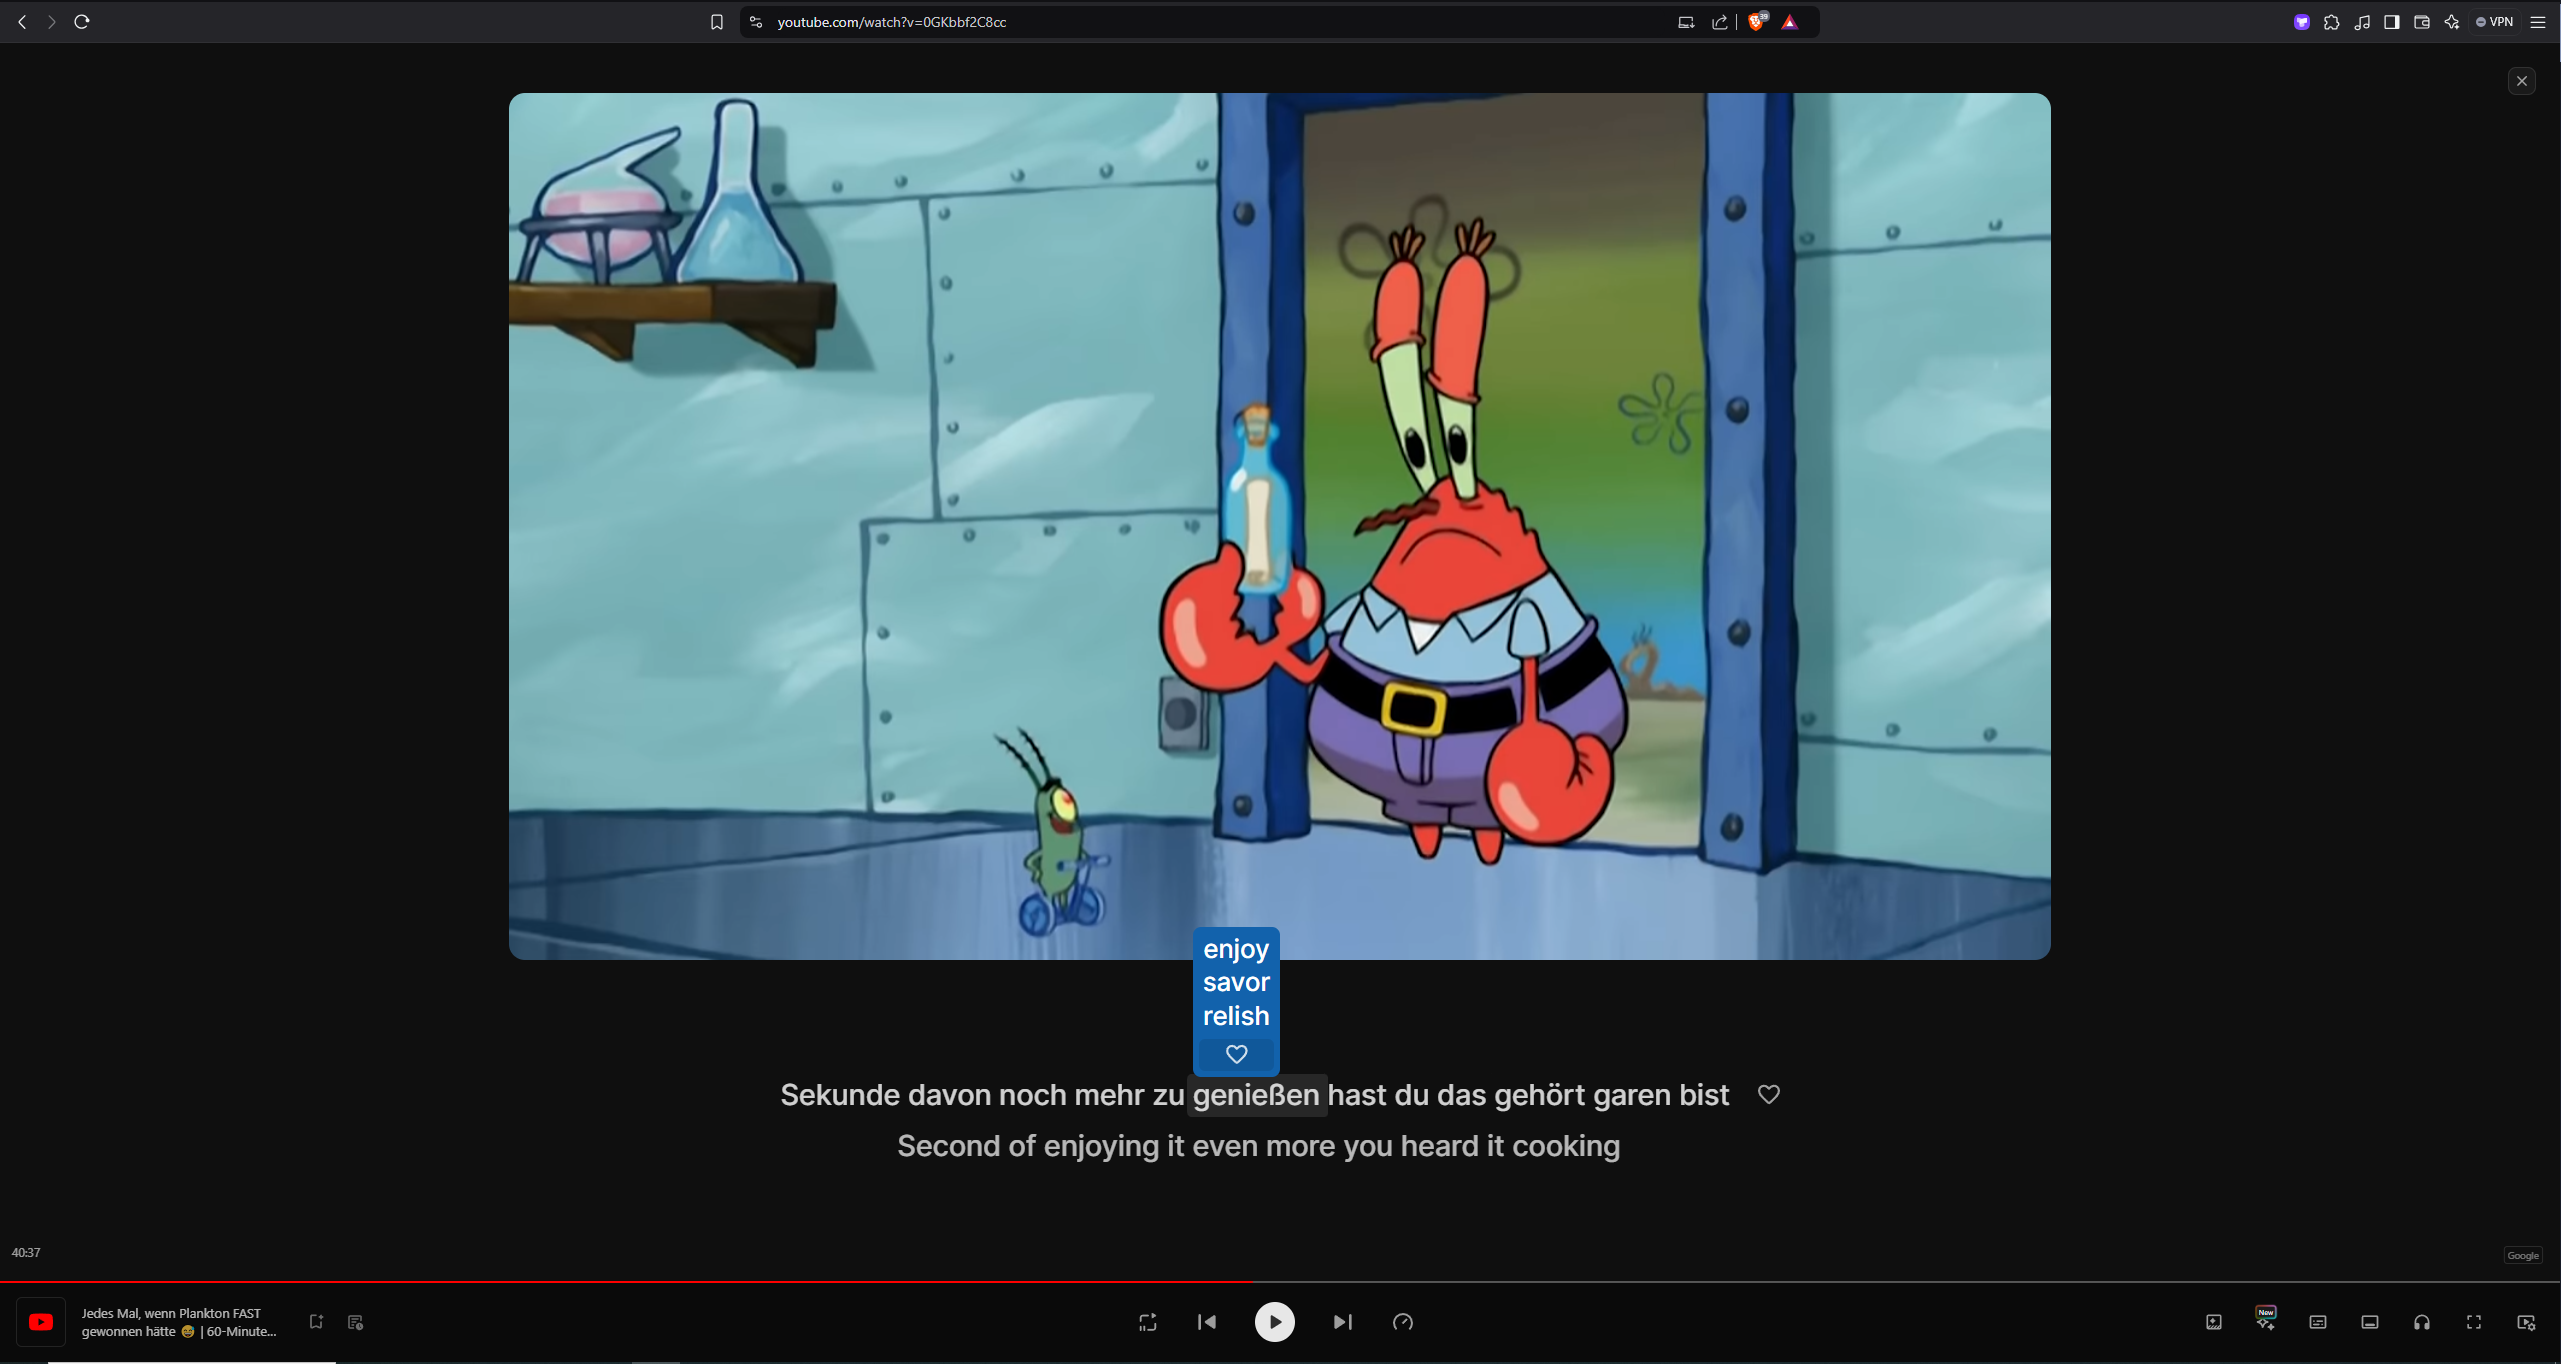
\includegraphics[width=0.8\textwidth]{IMAGE/Trancy.png}
    \caption{Interaktywne napisy na stronie Trancy}
    \label{fig:Trancy}
\end{figure}